\chapter{The Large Hadron Collider (LHC) and the ATLAS experiment.}
\minitoc

Particle physics requires to build a large machine for probing it theories. This a modern field of the physics, that pushes a limits of engineering. In this section an overview of the experimental setup, used to collect a data for this analysis will be given. The first section introduces an cutting edge of particle accelerators: LHC. In the send section an \atlas detector will be described. 

\section{The LHC and accelerator complex}

Large hadron collider is the largest accelerator in the world. It was build in Geneva, Switzerland and started its operation with the first collisions in 2009. It lies in a tunnel 27 kilometers in circumference. It operates with pp and Pb-Pb beams with centre-of-mass energies up to 14 GeV. It was designed to make a precise studies of Standard Model predictions and to search for a new physics beyond standard model, such as suppersymmetry. The heavy ion program serves a purpose of studying matter properties and a quark-gluon plasma.

Beams acceleration consists of several stages, as it shown in Fig. \ref{fig:LHC}. The beam source is a hydrogen gas or lead source in case of the heavy ion.  An electrical current is used to remove the electrons from each atom, and then the ion begin its ride through the only linear accelerator in the chain LINAC2, that accelerates protons up to 50 GeV or LINAC3 with up to 3.2 GeV/nucleon. The proton beams from linac are ejected into the PS booster, where they are further accelerated to 1.4 GeV.  During a heavy ion operations nucleons from LINAC3 are injected into the Low Energy Ion Ring (LEIR) and are accelerated up to 72.2 MeV/nucleon before injecting into PS.  The last steps before ejecting beams to the LHC are the rings of the Proton Synchrotron (PS) and Super Proton Synchrotron (SPC) that accelerates protons to 25 and 450 GeV respectively. The bunch structure of the beam is formed at PS step and has a nominal pattern of 39 groups of 72 bunches with time 25-50 ns time spacing. 

In LHC beams are accelerated up to 7 TeV ( yet 6.5 TeV achieved). The beams are circulating in opposite directions inside one of the 2 beam pipes, that are 6.3 cm in diameter. In order to bend beam trajectory, the pipes are surrounded by a 1232 superconducting dipole magnets. The superconducting cavities are used to accelerate the protons and maintain beam constant energy during the operation time. 

As most of the circular colliders, LHC has several experiments installed in the regions, where beams are intersecting, that allows them to collect data in parallel. The main experiments are:
\begin{description}
\item [ALICE] A large Ion Collider Experiment - a dedicated heavy ion detector, build to in the physics of strongly interacting matter, where a new phase of mater (quark-gluon plasma) is expected.
\item [ATLAS] A Toroidal LHC ApparatuS  is a largest particle detector build. It is a general purpose detector, that is used to study QCD and a Standard Model predictions and searches for a new physics. A detailed description of this detector is given in Sec. \ref{sec:ATLAS}.
\item [CMS] the Compact Muon Solenoid is an another multiple purpose detector at LHC, build with the different technologies in the respect to ATLAS.
\item [LHCb] the Large Hadron Collider beauty is specialized for measurement of heavy (charm and bottom) quark properties, that allows to study the parameters of CP violation.
\end{description}


\begin{figure}[!b]
\center{
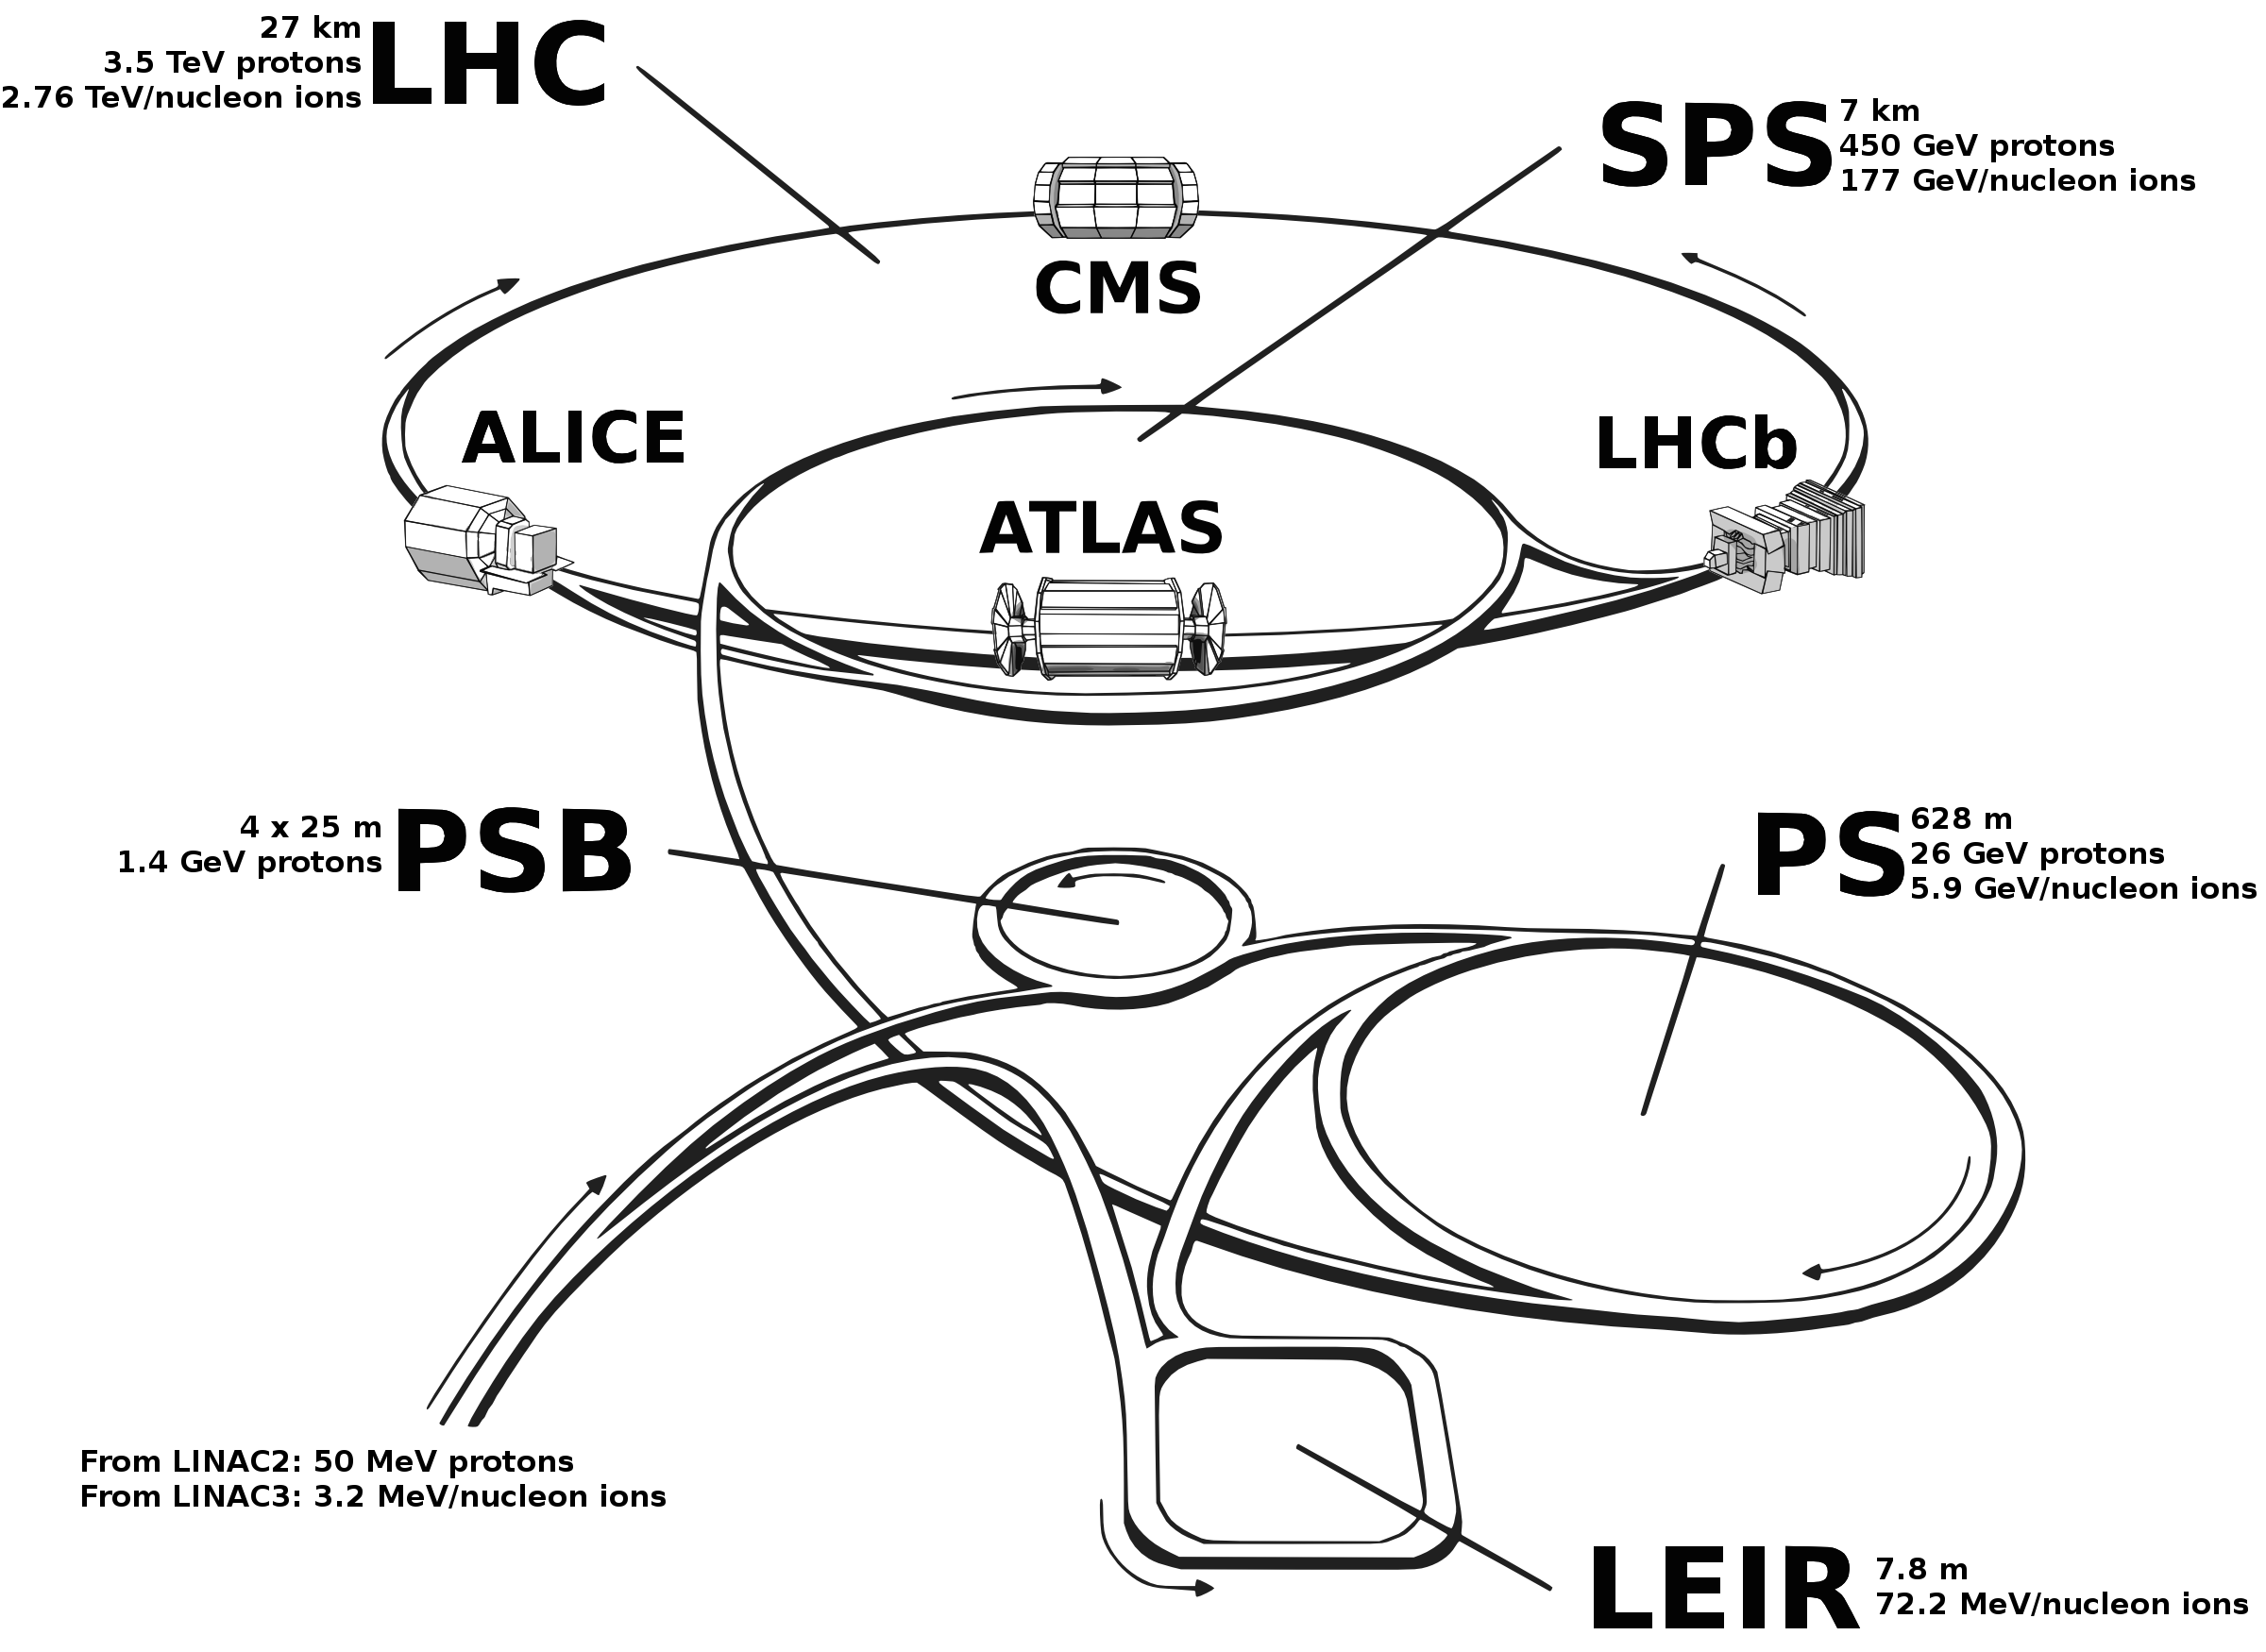
\includegraphics[width=0.8\textwidth]{LHCAtlas/cernAcceleratorComplex.png}
\caption{The LHC acceleration complex \cite{JetGoodson}}
\label{fig:LHC}}
\end{figure}

\section{The ATLAS experiment} \label{sec:ATLAS}

\begin{figure}[!tbp]
\center{
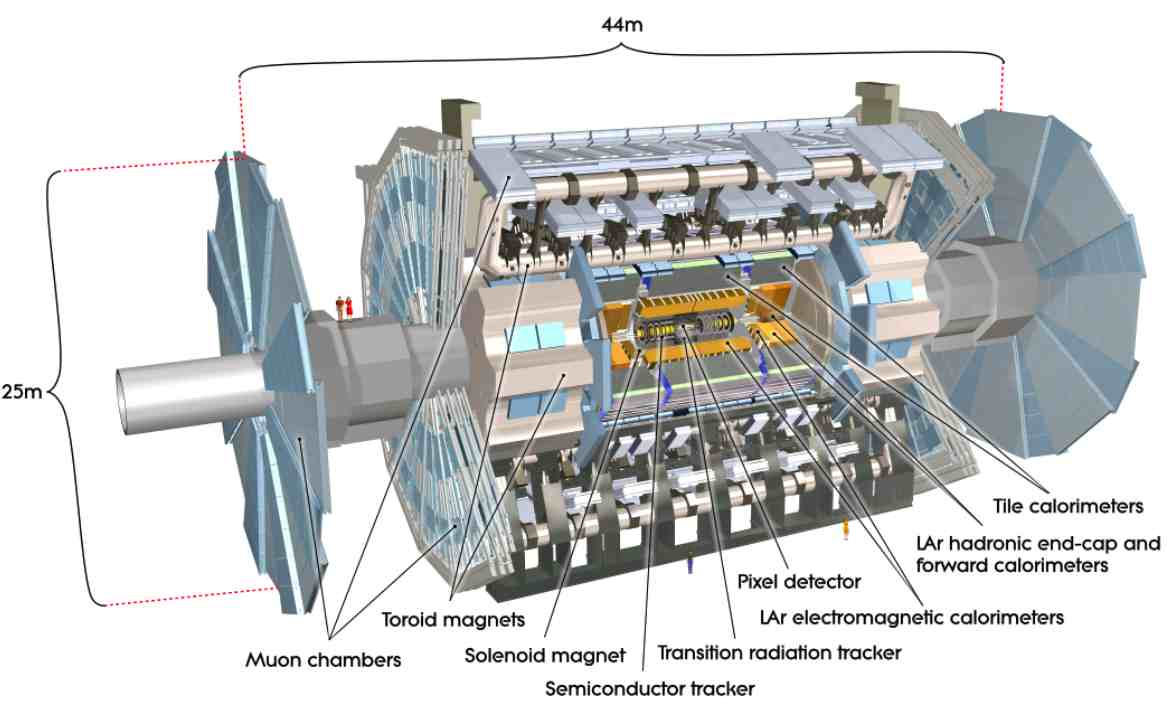
\includegraphics[width=1.0\textwidth]{LHCAtlas/ATLASDetector.png}
\caption{The ATLAS detector \cite{ATLASDetectorPlot}}
\label{fig:ATLASDet}}
\end{figure}
\atlas is a multi-purpose detector. It is used to preform different types of analysis. It is supposed to operate for a 2 decades. 

The physics goals and signatures of the particles are putting a strict set of requirements on \atlas detector. Heavy particles, born in pp collisions are expected to decay almost immediately. Thus their properties are measured only indirectly through their decay products, that should be detected and identified.  Good identification efficiency of photons, electrons and hadrons is achieved by the system of calorimeters. Because muons are minimum ionizing particles, they go further, than most of the particles, the special outer detector system is build. B-hadrons travel to the distance around 1 mm, producing a secondary vertex, so the vertex detectors near interaction point should be able to detect this. Neutrino from the decays are leaving the detector without interacting with it. However, it is possible to measure them through the energy imbalance in the detector. This means, that detector should cover a hermetically closed area near interaction point, so that no information is missed.  Radiation hardness for all of the detectors and electronic is required because of the LHC harsh environment. 

The \atlas detector can be divided into 3 main subdetectors, each serving its own purpose
\begin{itemize}
\item The Inner Detector (ID), that is used for tracking and precise measurement of particles momentum
\item The Calorimetry system that is used to measure the energies of electrons, photons and hadrons and to identify them
\item Muon system designed to detect muons and measure their parameters.
\end{itemize}

Each subdetector can be divided into 3 parts: the barrel region near the interaction point and end-cap in the forward directions.  The magnet system is used for tracking of charged particles for measurements of momentum and charge. The \atlas detector has 4 large superconducting magnet: solenoid, build around inner detector and 3 toroids (end-cap and forward) used for the muon spectrometer. 

\subsection{Coordinates and kinematic variables}
The detector shape motivates the choice of the coordinate system. It is natural to choose $z$ axis to be aligned with the beam, with the start in interaction point, while leaving x and y axis to be perpendicular to it. Because of detector symmetry along the beam z axis, the cylindrical coordinates are often used, with the radial distance $r=\sqrt{x^2+y^2}$ and the polar $\theta$ and azimuth $\phi$ angles.  

The direction of the particles can be quantified via rapidity:
\begin{equation}
y = ln \sqrt{\frac{E+p_z}{E-p_z}},
\end{equation}
where $E$ is the energy of the particle and $p_{z}$ is z component of the momentum. In the limit of the vanishing masses, this quantity is converges to another widely used variable called pseudorapidity:
\begin{equation}
\eta = - ln \Big[tan\Big(\frac{\theta}{2}\Big)\Big].
\end{equation}
It is preferred over the polar angle, because the differences in pseudorapidity is the Lorentz invariant along the boost in the beam direction. 

The spacial distance between two Lorentz vectors is defined as:
\begin{equation}
\Delta R = \sqrt{(\Delta\eta)^2+(\Delta\phi)^2}.
\end{equation}

The transverse momentum is defined as:
\begin{equation}
p_T=\sqrt{p_x^2+p_y^2},
\end{equation}
where $p_x$ and $p_y$ are the x and y components of the particle momentum. Because the incoming protons are alligned along the z axis, the total transverse momentum (together with non-interacting particles) in the detector should be fixed to 0. 

\subsection{Inner detector}

\begin{figure}[!tbp]
\center{
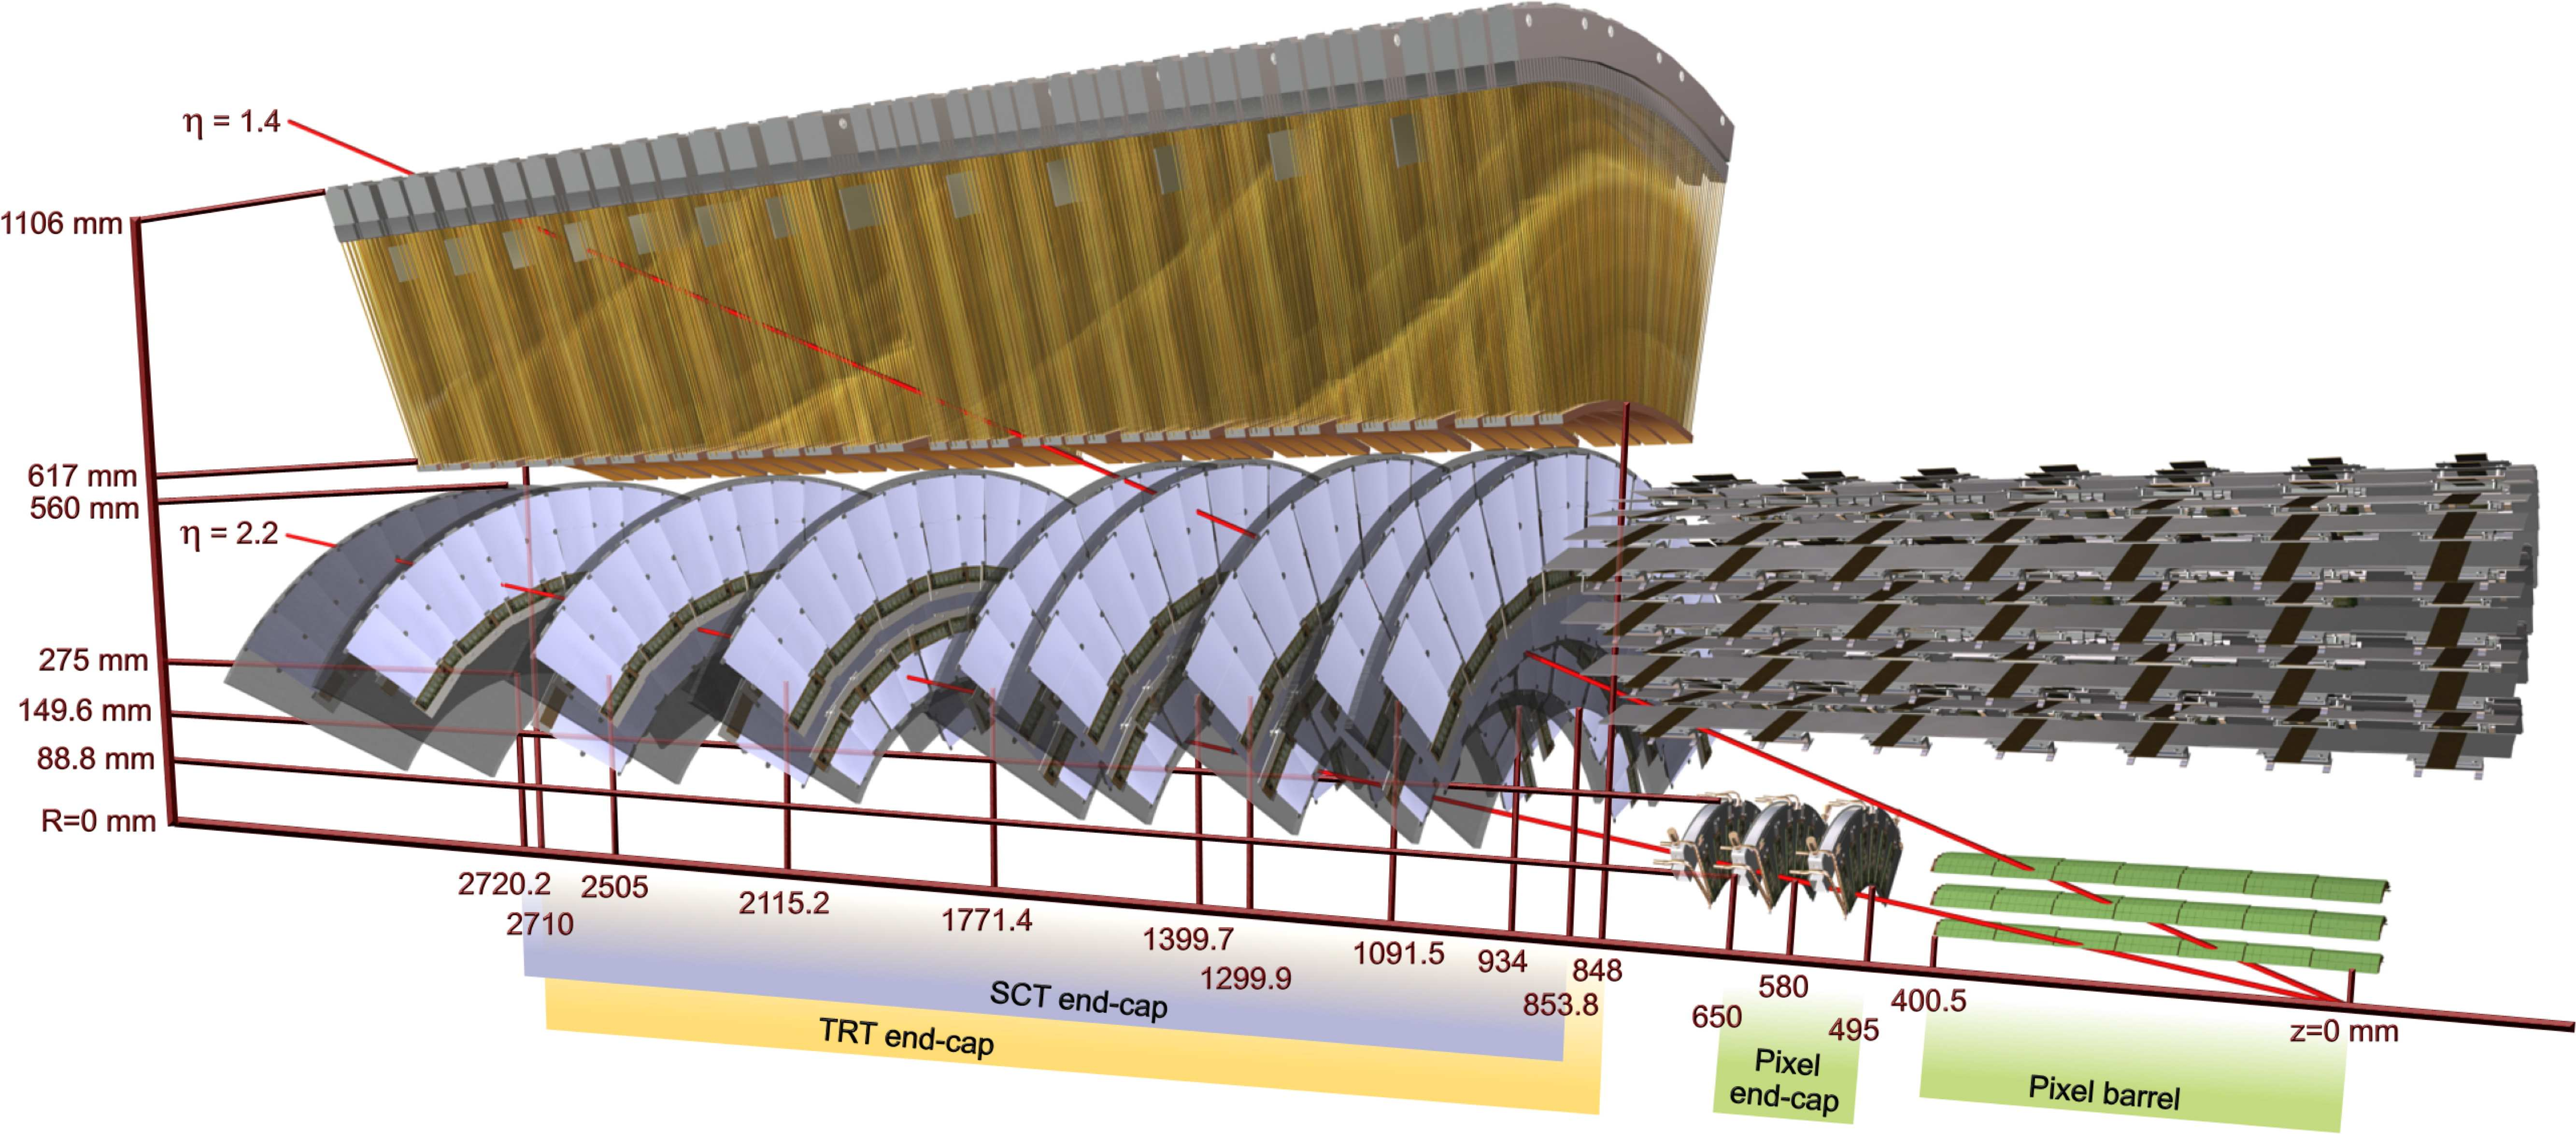
\includegraphics[width=1.0\textwidth]{LHCAtlas/FigID.pdf}
\caption{Cut-away view of the ATLAS Inner Detector. Drawing is showing the sensors and structural elements traversed by two charged tracks of 10GeV pT in the end-cap inner detector\cite{AtlasExperiment}}
\label{fig:ATLASID}}
\end{figure}

The Inner Detector (ID) is the closest to the interaction point detector system. It used for reconstruction of charged particles tracks and vertexes.  Approximately 1000 particles are emerging during one collision within Inner Detector (ID) acceptance ($| \eta |$ < 2.5). In order to achieve a good momentum and verex resolution it is required to use a high granularity detector. The layout of ID is shown in Fig. \ref{fig:ATLASID}. 

The inner detector consists of 3 sub-detectors:
\begin{itemize}
\item The precise reconstruction of vertexes with spacial resolution of 1 mm achieved because of the pixel detectors, placed close to the interaction point. The pixel detector consists of approximately 80.4 million readout channel placed in 3 barrel and 3 disk layers at the end of each barrel region.  Each pixel module made of the silicon layer and s lower layer of electronics. Charged particle, passing through the module, creates a movement of electron-hole pair, that causes a current in the readout electronics.
\item The silicon strip detector (SCT) consists of 6.3 million readout channel. It gives a significant contribution on a measurement of charged particle momentum, because of the large number of hits particle produce in the detector. It works in a similar way with pixel detector, however has a smaller precision. Each track crosses around 8 strip layers. 
\item Transition radiation tracker (TRT) consists of the straw tubes and provides the largest number of hits ( $\sim$ 36 per track). Each straw is a polimide drift tube 4 mm in a diameter. The tubes are placed parallel to the beam in the barrel region and radially in the wheels.
\end{itemize}

The combination of the precision measurments near the interaction point and big amount of hits at larger distances allows atlas to have a good precision of the coordinates measurements.

\subsection{Calorimeters}\label{sec:forwardCalo}
\begin{figure}[!tb]
\center{
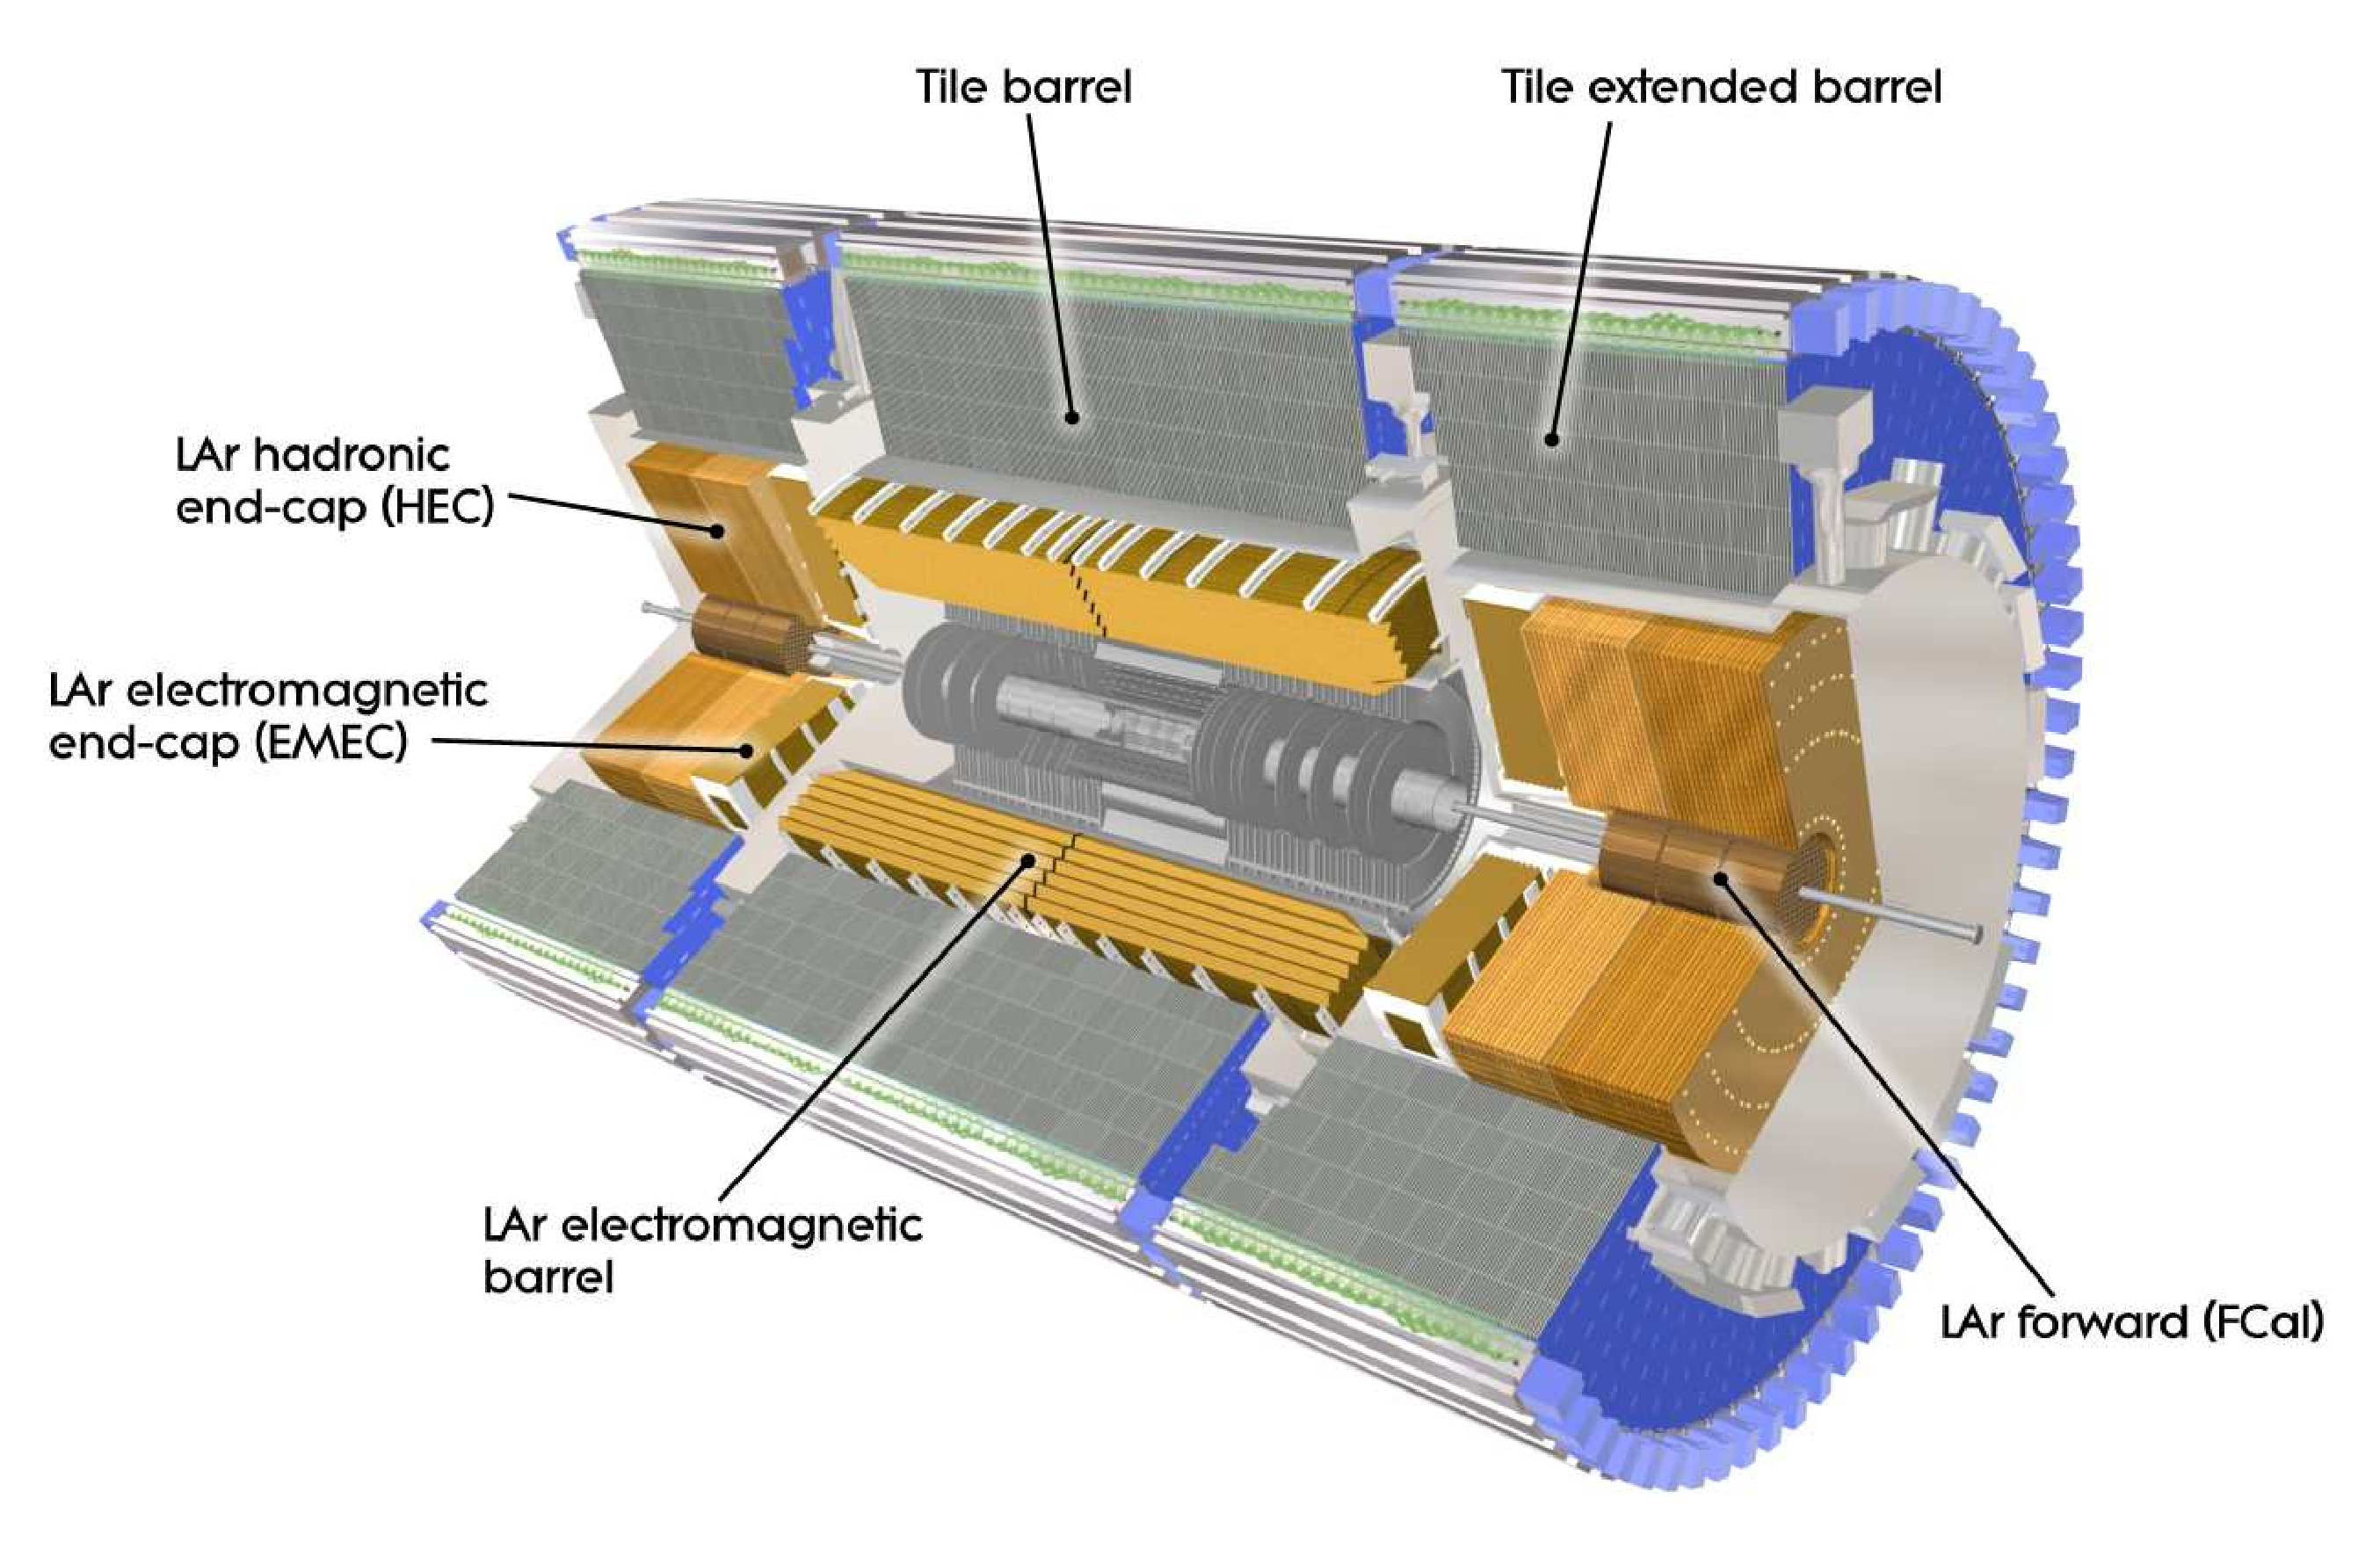
\includegraphics[width=1.0\textwidth]{LHCAtlas/Calorimeter.pdf}
\caption{Cut-away view of the ATLAS calorimeter system \cite{AtlasExperiment}}
\label{fig:ATLASCalo}}
\end{figure}

The calorimeter system is used to measure position and energy of particles from their deposits in the material.The general structure of \atlas calorimeter is shown in Fig. \ref{fig:ATLASCalo}. The calorimetric system consists of barrel ( 	$|\eta|$ < 3.2 ) and two end-cap parts ( 3.1 < $|\eta|$  < 4.9 ). The central part used of the high precision measurments, while the end-cap part has a coarser granularity and mostly used for jet reconstruction and \etmiss measurements. 

Particles, entering the calorimeter, produce a casecade of the secondary particles called a particle shower. Each shower is registered by the set of smallest structures of calorimeter providing the responce, called cells. Cell structure, called shower shape, differs for different types of particles and used for identification. Each calorimeter also has a dead material, that is used to absorb particles and does not produce any signal response. The full particle energy is reconstructed from the ratio between amount of energy absorbed in dead and active material.

In order to measure the energy of the particle properly, shower should be fully contained by the calorimeter. Since depth of the shower, caused by electomagnetic particle is significantly smaller, than depth of the hadronic shower, calorimeters are divided into two types: electromagnetic (EM) and hadronic. EM calorimeters are placed closer to the interaction point and has smaller amount of the dead material, compared to the hadronic calorimeters.

The central region calorimeters are required to have high granularity for combination with ID information and a precision measurement of photons and electrons. Forward part has aa smaller granularity and mostly used for jet reconstruction and missing transverse energy measurements.

\subsubsection{Electromagnetic calorimeter}
\begin{figure}[!tb]
\center{
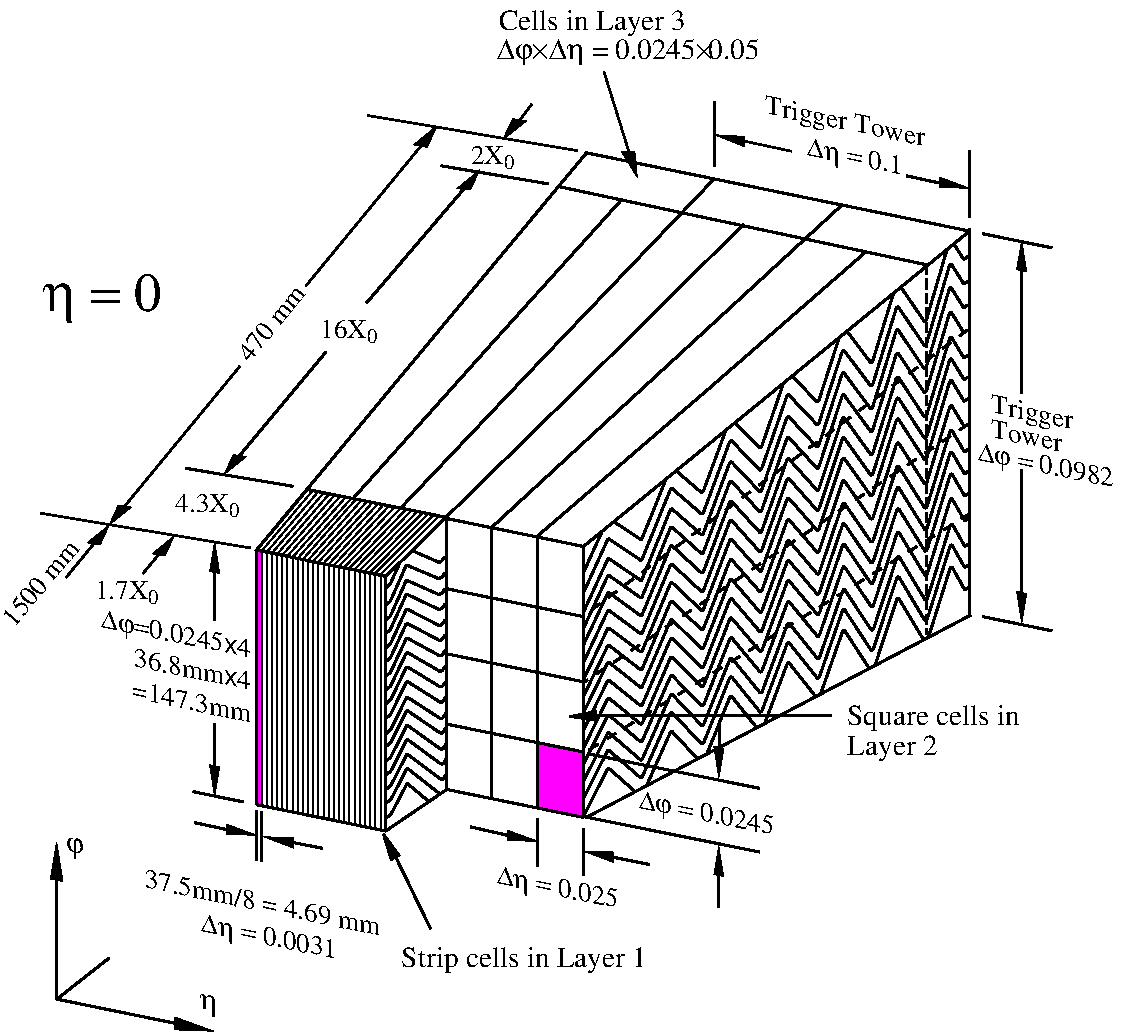
\includegraphics[width=0.7\textwidth]{LHCAtlas/BarellCalo.pdf}
\caption{The sketch of EMB module.  The granularity in $\eta$ and $\phi$ of the cells of each of the three layers and of the trigger towers is also shown \cite{AtlasExperiment}}
\label{fig:ATLASCaloEM}}
\end{figure}

The main purpose of electromagnetic calorimeter is to measure energies of electrons and photons. The EM showers starts from initial high-energy electron and photon entering the calorimeter. High-energy photons are loosing their energy via production of electron-positron pairs, while electrons and positrons are emiting photons via Bremstrallung. These two processes continues till the photon reaches the pair production threshold. 

The EM calorimeter consists of a barrel part (EM barrel = EMB) and two symmetric end-caps (EM end-cap = EMEC), that cover a range of pseudorapidity $|\eta|<1.475$ and $1.5 < |\eta|<3.2$ respectively. These calorimeters have an accordion stucture, as shown in Fig. \ref{fig:ATLASCaloEM}. This geometry allows to have a full coverage in $\phi$ coordinate.
It consists of the layers of lead/steel interplaced with liquid argon, that acts as a sensitive material, and electronics.

There are four samplings in EMB calorimeter, as showed in Fig. \ref{fig:ATLASCaloEM}:
\begin{description}
\item [presampler] A single layer of LAr without dead material in front of it. It allows to correct for the energy losses in front of the calorimeter. 
\item [1st sampling] The first layer has a fine segmentation in $\eta$ with thin $\eta$ strips with size $\Delta \eta \times \Delta \phi = 0.0031 \times 0.098$. Because of the resolution this layer provides an information for $\gamma$ and $\pi^0$ separation.
\item [2nd sampling] The majority of the energy is deposited in the second sampling layer. It consists of the square cells with size $\Delta \eta \times \Delta \phi = 0.0245 \times 0.0245$.
\item [3rd sampling] Just the highest energy electrons are reaching the third layer, therefore it has a bigger cell size.
\end{description} 

Each wheel of the EMEC calorimeter consists of the 2 co-axial wheels: Inner Wheel (IW) and Outer Wheel (OW). Each endcap wheel is divided into 8 wedge-shaped modules.  <MORE ABOUT EMEC.

<Add about trigger>

\subsubsection{Hadronic calorimeters}

The mechanism of hadronic shower development differs from the electromagnetic one. The main physical processes, that are determining the shower development are: hadron production, nuclear deexcitation and pion and muon decays. It usually takes longer to develop a hadronic shower, than an EM one.

The \atlas hadronic calorimeter consists of the tile and liquid argon Hadronic End-cap Calorimeter (HEC). The forward part of the hadronic calorimeter will be discussed separately.

The tile calorimeter placed right after the EMEC and covers a pseudorapidity range up to $|\eta|$<1.0 in the barrel region and 0.8<$|\eta|$<1.7 in the 2 end-caps. It is a sampling calorimeter with steel acting as a dead material and scintilator ties for a senstive material. The readout from scintillator performed using the wavelength shifting fibers.  The readout cells are build by grouping the fibers into the photomultiplier. Granularity of the detector

The HEC calorimeter uses a liquid argon as a sensitive matrial and shares the same LAr cryostat with EMEC. The copper-plate are acting as an absorbers with a flat-plate design. The size of the cell in HEC is $\Delta \eta \times \Delta \phi = 0.1 \times 0.1$ for $|\eta|$<2.5 and $\Delta \eta \times \Delta \phi = 0.2 \times 0.2$ for forward region $|\eta|$>2.5


\subsubsection{Forward calorimeter}


\begin{figure}[!tbp]
\begin{minipage}[h]{0.45\linewidth}
\center{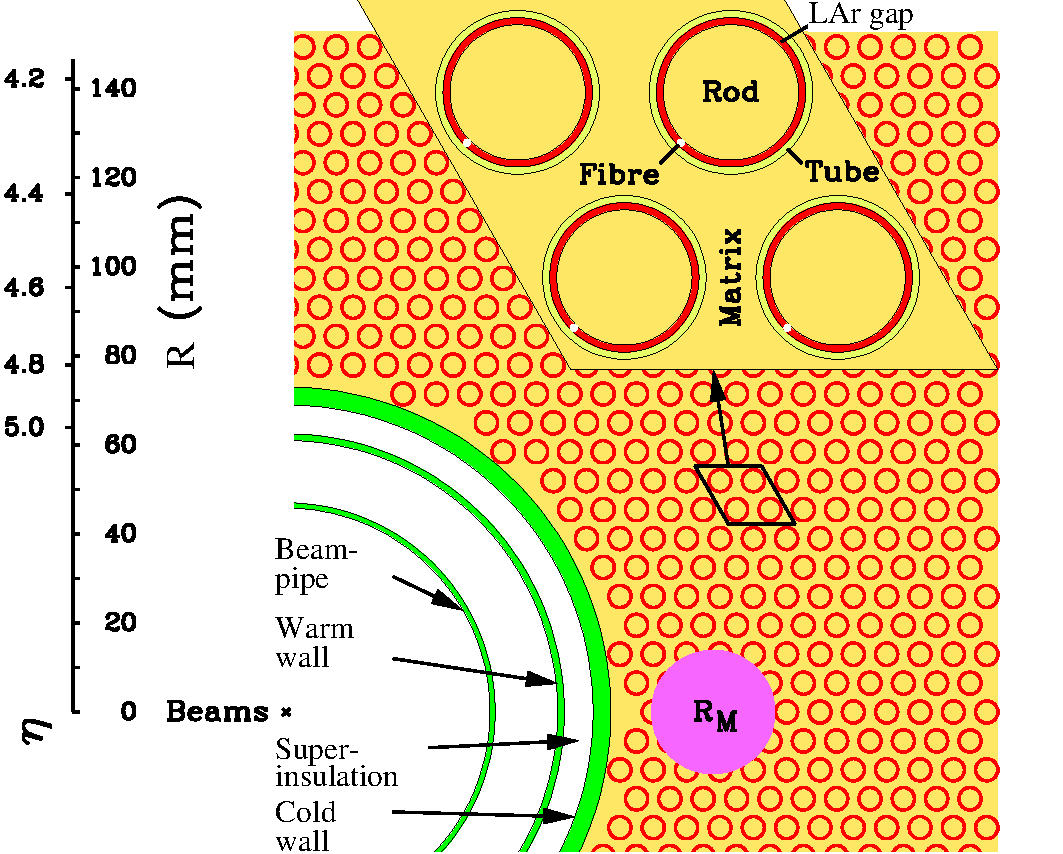
\includegraphics[width=1.\linewidth]{LHCAtlas/FCAL.pdf} }
\caption{Electrode structure of FCAL1 with the matrix of copper plates and copper tubes and rods with the LAr gap for electrodes \cite{AtlasExperiment}}
\label{fig:FCALModel}
\end{minipage}
\hfill
\begin{minipage}[h]{0.49\linewidth}
\center{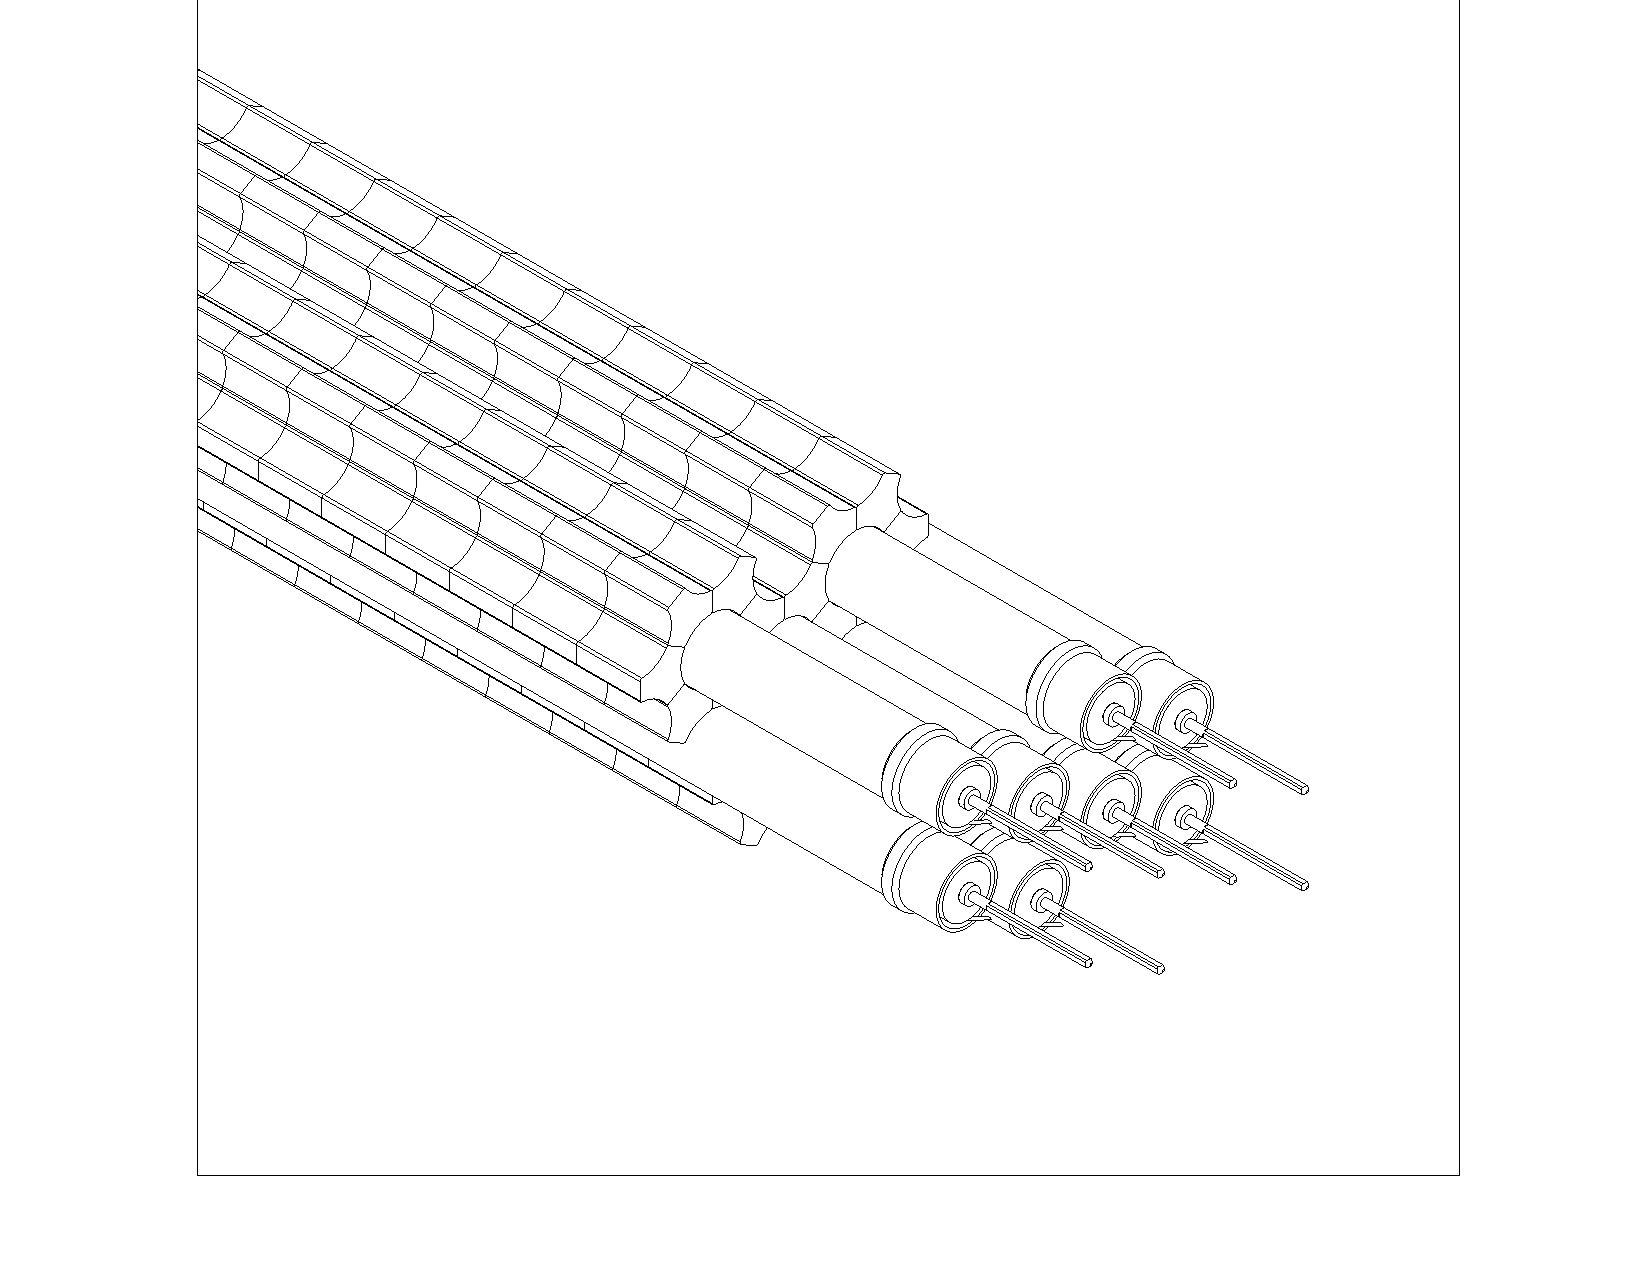
\includegraphics[width=1.\linewidth]{LHCAtlas/FCALMod.pdf}}
\caption{View of the FCAL hadronic module absorber matrix, including a set of tungsten rods and copper tubes surrounded by 1 cm long tungsten slugs\cite{AtlasExperiment}}
\label{fig:FCAL2}
\end{minipage}
\end{figure}


The forward calorimeter (FCAL) is placed in the same cryostat with EMEC and covers the range of pseudorapidity 3.1 < $|\eta|$ < 4.9. It is placed 4.7 m away from the interaction point and imposed for a high fluxed. This motivates the choice of detector design with small amount of the sensitive material.  The FCAL module consists of the co-axial copper rod and anode tube, separated by the wire around the rod. The LAr fills the gap between rod and anode. Small size of the gaps allows to have faster signal transfer together with avoiding signal degration caused by distortion of the electric field in the gap (some reference). The structure of one of the FCAL calorimeters is shown in Fig. \ref{fig:FCALModel}.

The FCAL is divided into 3 modules: one electromagnetic FCAL1 and 2 hadronic FCAL2 and FCAL3. Parameters of these modules are summarized in Tab. \ref{tab:FCALParam}. In hadronic modules it was decided to use a tungsten instead of the copper in order to optimize the high absorption length. These modules a similar to the FCAL1, except for the use of tungsten rods instead of the copper rods. The space between the end-plates and tubes is filled with tungsten slugs, as shown in Fig. \ref{fig:FCAL2}.

The electrodes are forming the readout cells from the group of four, six and nine for FCAL1, FCAL2 anf FCAL3 respectivelly. The granularity of the detector is about $\Delta \eta \times \Delta \phi \approx 0.2 \times 0.2$

\begin{table}[!tbp]
\caption{Table of parameters for the three FCAL modules}
\label{tab:FCALParam}
\begin{center}
\begin{tabular}{ l | c | c | c | c | c }
\hline
Calorimeter & Type & Absorber & Gap width & Number & Number \\
 & & &  ($\mu m$)  & of electrodes & of readout channels \\
\hline
\hline
FCAL1 &  electromagnetic & coper & 250 & 12 260 & 1008\\
FCAL2 &  Hadronic & tungsten & 375 & 10 200 & 500\\
FCAL2 &  Hadronic & tungsten & 500 & 8 224 & 254\\
\hline
\end{tabular}
\end{center}
\end{table}

\subsection{Muon spectrometer}\label{sec:MuonSys}
The muon trajectories are already measured in the ID, however for a high $P_{T}$ muons it could be difficult to make a precise determination of charge and momentum. The Muon Spectrometer (MS) provides an information at a much larger scales to measure the bending of the trajectory because of the magnetic field. The MS is placed in the most outer part of the \atlas detector, behind the calorimeters. The amount of the mateiral in front of the MS is adjusted so, that it can be assumed, that all of the particles entering the it are muons. 

The muon spectrometer covers the area up to $|\eta|$ < 2.7 and allows to trigger on these particles in the range $|\eta|$ < 2.4. The precision tracking is performed by the Monitored Drift Tubes (MDT). The MDT consists of 8 layers of the drift tubes and allowing to have a resolution of 80 $\mu$m per tube or 35 $\mu$m per chamber. In addition, in forward region 2.0 < $|\eta|$ < 2.7, the Cathode-Strip Chambers (CSC) are used. The CSC are the multiwire proportional chambers and giving a resolution 40 $\mu$m in the bending plane and 5 mm in the transverse plane.

The trigger system in muon spectrometer is composed from the fast detectors namely Resistive Plate Chambers (RPC) and Thin Gap Chambers (TGC) in the barrel($|\eta|$ < 1.05) and end-cap (1.05 < $|\eta|$ < 2.4) regions respectively. 

\begin{figure}[!tb]
\center{
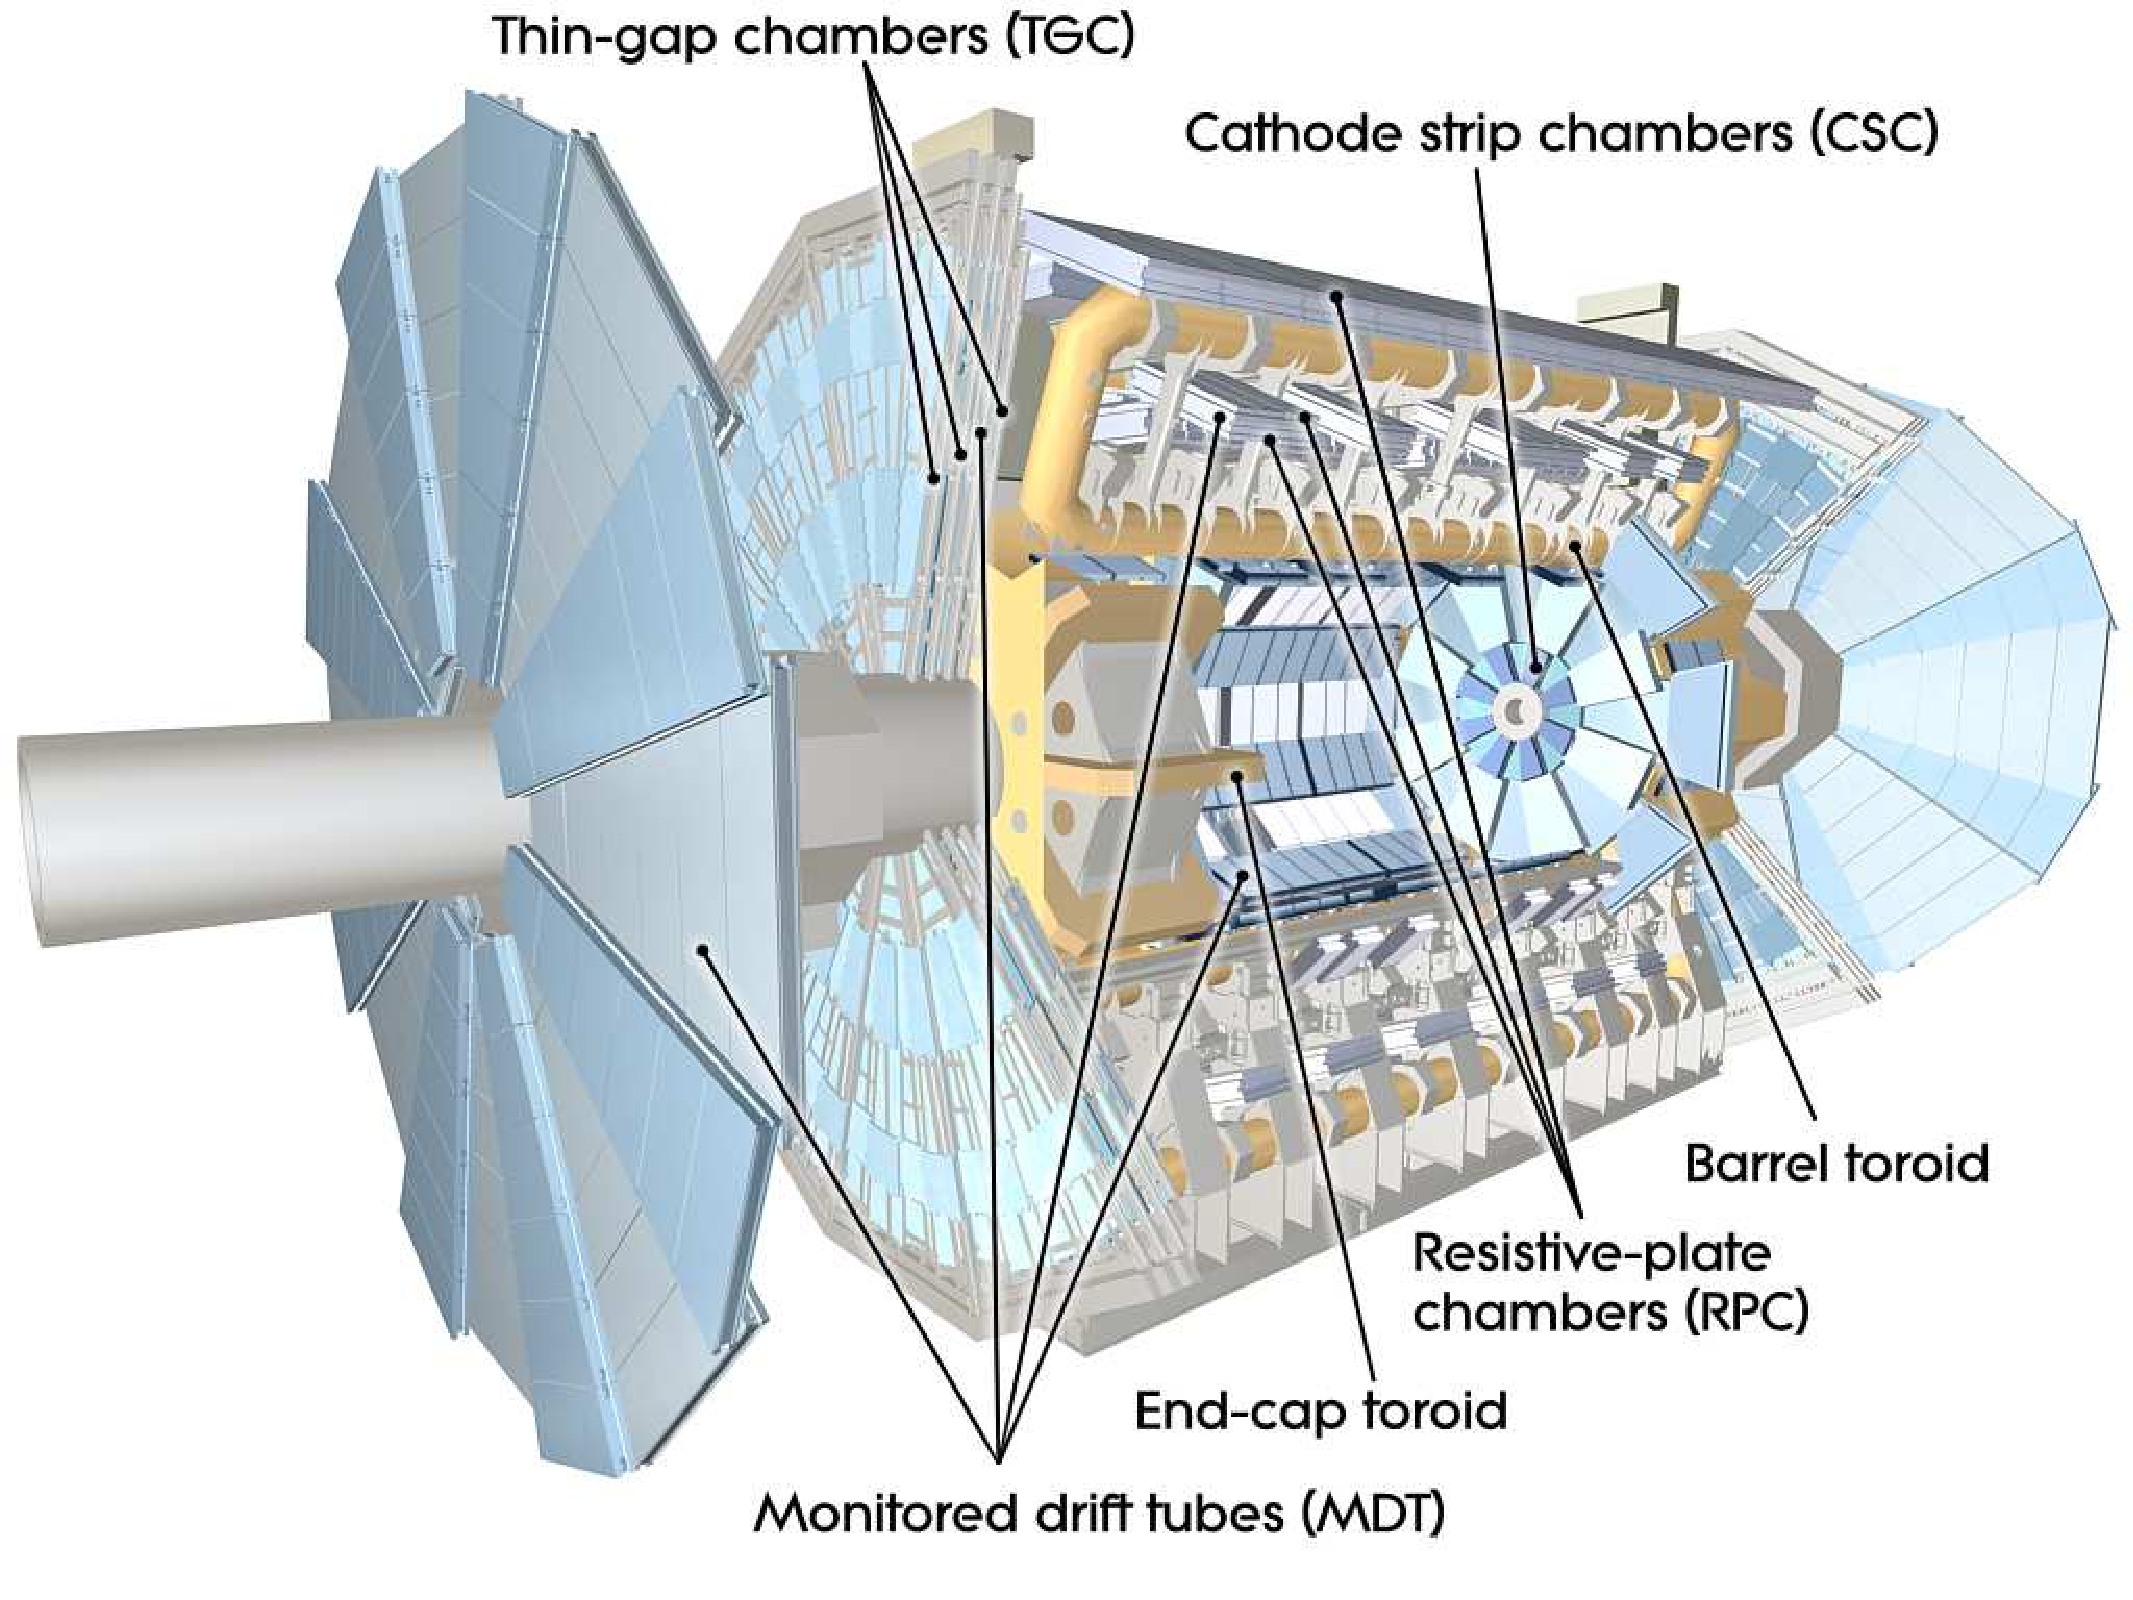
\includegraphics[width=0.8\textwidth]{LHCAtlas/MuonSystem.pdf}
\caption{Cut-away view of the ATLAS muon system. \cite{AtlasExperiment}}
\label{fig:ATLASMuon}}
\end{figure}

\subsection{Trigger system}
Processing and storing of the events is a difficult task at LHC. The collision frequency at LHC is 40 MHz. The full readout information of 1 second of operation requires requires 1 Tb of storage space. However, the events of interest (such as production of bosons) makes just a small fraction out of these events. The trigger system used for reducing the information stored, while leaving "interesting" events untouched. It covers a range of pseudorapidity up to 2.5.

The trigger system can be divided into 3 levels of selection:
\begin{description}
\item[Level-1] The first level trigger should have a high operation speed, so it uses reduced-granulatrity information form Recistive Plate Chambers (RPC) and Thin-Gap Chambers (TGC) and calorimeter systems. It searches for leptonic and hadronic signatures (or large total transverse energy) in the detector. This trigger allows to reduce a rate, that can be handled by a readout electronics (~ 75 kHz).
\item[Level-2] The second level trigger analyses in more details Regions-of-Interest (RoI's) identified by Level-1 trigger. It uses an information on RoI's such as energy and a position of clusters to further reduce the data trasnfered. The Level-2 event rate is below 3.5 kHz, with processing time around 30 ms in average.
\item[High-Level Trigger (HLT)] The last level selection is performed offline on large farm of CPUs. It analyses a full information from detectors to refine a tirgger selections. The additional information from tracking allows to improve particle identification and distinguish electrons and photons. About 200 events per second are left after the HLT and transmitted to the permanent storage.
\end{description}

The data aquisiton system (DAQ) recieves information from the readout electronics at the L1 trigger rate and  transfers the data to L2. After passing the L2 selection criteria the event is build and transmitted to HLT.

\section{Luminosity measurement}

One of the main components, characterizing the collider is the instantaneous luminosity $\lumi(t)$ delivered, that is defined as a propotional factor between the cross-section $\sigma_p$ and number of interactions per second $\frac{dR}{dt}$, as :
\begin{equation}
\frac{dR}{dt}= \lumi(t) \times \sigma_p (cm^{-2}s^{-1}).
\end{equation}
This value is a relativistic invariant and independent on physical reaction.

In case of LHC, that performs  head-on collisions of particle bunches, it could be calculated as per beam value:
\begin{equation}
\lumi = \frac{N_p^2 N_b f_{\textrm{rev}}}{4\pi  \sigma_x \sigma_y}F , 
\end{equation}
where $N_{p}$ is the number of protons per beam, $N_b$ - number of bunches, $f_{\textrm{rev}}$ is the revolution frequency, $\sigma_x$ and $\sigma_y$ are the horizontal and vertical beam profile widths. The factor F is coming from the beam crossing angle. In 2012, at 8 TeV centre-of-mass energy, the LHC machine was able to reach an instanteneous luminosity $7.7\times10^{33}\, [cm^{-2}s^{-1}]$.  

The \atlas experiment uses several detectors to measure the recorded luminosity. The Beam Condition Monitor (BCM) monitores a beam parameters close to the interaction point and allows to measure bunch intensities. In the forward region a special detector for a luminosity measurements is placed: the LUCID (LUminosity measurement using Cerenkov Integrating Detector) detector. It detects the intelastic scattering.